\chapter{Gretl and \TeX}
\label{gretltex}


\section{Introduction}
\label{tex-intro}

\TeX\ --- initially developed by Donald Knuth of Stanford University
and since enhanced by hundreds of contributors around the world --- is
the gold standard of scientific typesetting.  \app{Gretl} provides
various hooks that enable you to preview and print econometric results
using the \TeX\ engine, and to save output in a form suitable for
further processing with \TeX.

This chapter explains the finer points of \app{gretl}'s \TeX-related
functionality.  The next section describes the relevant menu items;
section~\ref{tex-tune} discusses ways of fine-tuning \TeX\ output; and
section~\ref{tex-install} gives some pointers on installing (and
learning) \TeX\ if you do not already have it on your computer.  (Just
to be clear: \TeX\ is not included with the \app{gretl} distribution;
it is a separate package, including several programs and a large
number of supporting files.)

Before proceeding, however, it may be useful to set out briefly the
stages of production of a final document using \TeX.  For the most
part you don't have to worry about these details, since, in regard to
previewing at any rate, \app{gretl} handles them for you.  But having
some grasp of what is going on behind the scences will enable you to
understand your options better.

The first step is the creation of a plain text ``source'' file,
containing the text or mathematics to be typset, interspersed with
mark-up that defines how it should be formatted.  The second step is
to run the source through a processing engine that does the actual
formatting.  Typically this is either:
\begin{itemize}
\item a program called \app{latex} that generates so-called DVI
  (device-independent) output, or
\item a program called \app{pdflatex} that generates PDF
  output.\footnote{Experts will be aware of something called ``plain
    \TeX'', which is processed using the program \app{tex}.  The great
    majority of \TeX\ users, however, use the \LaTeX\ macros,
    initially developed by Leslie Lamport.  \app{Gretl} does not
    support plain \TeX.}
\end{itemize}

For previewing, one uses either a DVI viewer (typically \app{xdvi} on
GNU/Linux systems) or a PDF viewer (typically Adobe's Acrobat Reader
or \app{xpdf}), depending on how the source was processed.  If the DVI
route is taken, there's then a third step to produce printable output,
typically using the program \app{dvips} to generate a PostScript file.
If the PDF route is taken, the output is ready for printing without
any further processing.

On the MS Windows and Mac OS X platforms, \app{gretl} calls
\app{pdflatex} to process the source file, and expects the operating
system to be able to find the default viewer for PDF output; DVI is
not supported.  On GNU/Linux the default is to take the DVI route, but
if you prefer to use PDF you can do the following: select the menu
item ``Tools, Preferences, General'' then the ``Programs'' tab.  Find
the item titled ``Command to compile TeX files'', and set this to
\texttt{pdflatex}.  Make sure the ``Command to view PDF files'' is set
to something appropriate.  

\section{\TeX-related menu items}
\label{tex-menus}

\subsection{The model window}

The fullest \TeX\ support in \app{gretl} is found in the GUI model
window.  This has a menu item titled ``LaTeX'' with sub-items
``View'', ``Copy'', ``Save'' and ``Equation options'' (see
Figure~\ref{fig:latex-menu}).  

\begin{figure}[htbp]
  \caption{\LaTeX\ menu in model window}
  \label{fig:latex-menu}
  \begin{center}
    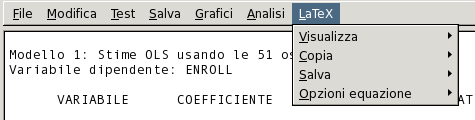
\includegraphics[scale=0.75]{figures/latex_menu}
  \end{center}
\end{figure}

The first three sub-items have branches titled ``Tabular'' and
``Equation''.  By ``Tabular'' we mean that the model is represented in
the form of a table; this is the fullest and most explicit
presentation of the results.  See Table~\ref{tab:mod1} for an example;
this was pasted into the manual after using the ``Copy, Tabular'' item
in \app{gretl} (a few lines were edited out for brevity).

\begin{table}[htbp]
\caption{Example of \LaTeX\ tabular output}
\label{tab:mod1}
\begin{center}

Model 1: OLS estimates using the 51 observations 1--51\\
Dependent variable: ENROLL\\

\vspace{1em}

\begin{tabular*}{.8\textwidth}{@{\extracolsep{\fill}}
l% col 1: varname
  D{.}{.}{-1}% col 2: coeff
    D{.}{.}{-1}% col 3: sderr
      D{.}{.}{-1}% col 4: t-stat
        D{.}{.}{4}}% col 5: p-value (or slope)
Variable &
  \multicolumn{1}{c}{Coefficient} &
    \multicolumn{1}{c}{Std.\ Error} &
      \multicolumn{1}{c}{$t$-statistic} &
        \multicolumn{1}{c}{p-value} \\[1ex]
const &
  0.241105 &
    0.0660225 &
      3.6519 &
        0.0007 \\
CATHOL &
  0.223530 &
    0.0459701 &
      4.8625 &
        0.0000 \\
PUPIL &
  -0.00338200 &
    0.00271962 &
      -1.2436 &
        0.2198 \\
WHITE &
  -0.152643 &
    0.0407064 &
      -3.7499 &
        0.0005 \\
\end{tabular*}

\vspace{1em}

\begin{tabular}{lD{.}{.}{-1}}
Mean of dependent variable & 0.0955686 \\
 S.D. of dependent variable & 0.0522150 \\
Sum of squared residuals & 0.0709594 \\
Standard error of residuals ($\hat{\sigma}$) & 0.0388558 \\
Unadjusted $R^2$ & 0.479466 \\
Adjusted $\bar{R}^2$ & 0.446241 \\
$F(3, 47)$ & 14.4306 \\
\end{tabular}
\end{center}
\end{table}

The ``Equation'' option is fairly self-explanatory --- the results are
written across the page in equation format, as below:

%%% the following needs the amsmath LaTeX package

\begin{gather}
\widehat{\rm ENROLL} = 
\underset{(0.066022)}{0.241105}
+\underset{(0.04597)}{0.223530}\,\mbox{CATHOL}
-\underset{(0.0027196)}{0.00338200}\,\mbox{PUPIL}
-\underset{(0.040706)}{0.152643}\,\mbox{WHITE}
 \notag \\
T = 51 \quad \bar{R}^2 = 0.4462 \quad F(3,47) = 14.431 \quad \hat{\sigma} = 0.038856\notag \\
\centerline{(standard errors in parentheses)} \notag
\end{gather}

The distinction between the ``Copy'' and ``Save'' options (for both
tabular and equation) is twofold.  First, ``Copy'' puts the \TeX\
source on the clipboard while with ``Save'' you are prompted for the
name of a file into which the source should be saved.  Second, with
``Copy'' the material is copied as a ``fragment'' while with ``Save''
it is written as a complete file.  The point is that a well-formed
\TeX\ source file must have a header that defines the
\texttt{documentclass} (article, report, book or whatever) and tags
that say \verb|\begin{document}| and \verb|\end{document}|.  This
material is included when you do ``Save'' but not when you do
``Copy'', since in the latter case the expectation is that you will
paste the data into an existing \TeX\ source file that already has the
relevant apparatus in place.

The items under ``Equation options'' should be self-explanatory: when
printing the model in equation form, do you want standard errors or
$t$-ratios displayed in parentheses under the parameter estimates?
The default is to show standard errors; if you want $t$-ratios, select
that item.  

\subsection{Other windows}

Several other sorts of output windows also have \TeX\ preview, copy
and save enabled.  In the case of windows having a graphical toolbar,
look for the \TeX\ button.  Figure~\ref{fig:tex-icon} shows this icon
(second from the right on the toolbar) along with the dialog that
appears when you press the button.

\begin{figure}[htbp]
  \caption{\TeX\ icon and dialog}
  \label{fig:tex-icon}
    \begin{center}
      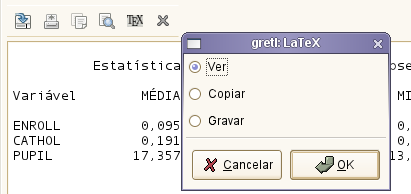
\includegraphics[scale=0.75]{figures/texdialog} 
    \end{center}
\end{figure}

One aspect of \app{gretl}'s \TeX\ support that is likely to be
particularly useful for publication purposes is the ability to produce
a typeset version of the ``model table'' (see
section~\ref{model-table}).  An example of this is shown in
Table~\ref{tab:modeltab}.

\begin{table}[htbp]
\caption{Example of model table output}
\label{tab:modeltab}
\begin{center}
OLS estimates\\
Dependent variable: ENROLL \\
\vspace{1em}

\begin{tabular}{lccc}
 & Model 1  & Model 2  & Model 3 \\  [6pt] 
const & $\,\,$0.2907$^{**}$ & $\,\,$0.2411$^{**}$ & 0.08557 \\
& \footnotesize{(0.07853)} & \footnotesize{(0.06602)} & \footnotesize{(0.05794)} \\ [4pt] 
CATHOL & $\,\,$0.2216$^{**}$ & $\,\,$0.2235$^{**}$ & $\,\,$0.2065$^{**}$ \\
& \footnotesize{(0.04584)} & \footnotesize{(0.04597)} & \footnotesize{(0.05160)} \\ [4pt] 
PUPIL & $-$0.003035 & $-$0.003382 & $-$0.001697 \\
& \footnotesize{(0.002727)} & \footnotesize{(0.002720)} & \footnotesize{(0.003025)} \\ [4pt] 
WHITE & $\,\,$$-$0.1482$^{**}$ & $\,\,$$-$0.1526$^{**}$ & \\
& \footnotesize{(0.04074)} & \footnotesize{(0.04071)} & \\ [4pt] 
ADMEXP & $-$0.1551 & & \\
& \footnotesize{(0.1342)} & & \\ [4pt] 
$n$ & 51 & 51 & 51 \\
$\bar R^2$ & 0.4502 & 0.4462 & 0.2956 \\
$\ell$ & 96.09 & 95.36 & 88.69 \\
\end{tabular}

\vspace{1em}
Standard errors in parentheses\\
{}* indicates significance at the 10 percent level\\
{}** indicates significance at the 5 percent level\\
\end{center}
\end{table}


\section{Fine-tuning typeset output}
\label{tex-tune}

There are two aspects to this: adjusting the appearance of the output
produced by \app{gretl} in \LaTeX\ preview mode, and incorporating
\app{gretl}'s output into your own \TeX\ files.

As regards preview mode, you can control the appearance of
\app{gretl}'s output using a file named \verb+gretlpre.tex+, which
should be placed in your \app{gretl} user directory (see the
\emph{Gretl Command Reference}).  If such a file is found, its
contents will be used as the ``preamble'' to the \TeX\ source.  The
default value of the preamble is as follows:
    
\begin{code}
      \documentclass[11pt]{article}
      \usepackage[latin1]{inputenc}
      \usepackage{amsmath}
      \usepackage{dcolumn,longtable}
      \begin{document}
      \thispagestyle{empty}
\end{code}

Note that the \verb+amsmath+ and \verb+dcolumn+ packages are required.
(For some sorts of output the \verb+longtable+ package is also
needed.)  Beyond that you can, for instance, change the type size or
the font by altering the \texttt{documentclass} declaration or
including an alternative font package.

In addition, if you should wish to typeset \app{gretl} output in more
than one language, you can set up per-language preamble files.  A
``localized'' preamble file is identified by a name of the form
\verb|gretlpre_xx.tex|, where \texttt{xx} is replaced by the first two
letters of the current setting of the \texttt{LANG} environment
variable.  For example, if you are running the program in Polish,
using \verb|LANG=pl_PL|, then \app{gretl} will do the following when
writing the preamble for a \TeX\ source file.

\begin{enumerate}
\item Look for a file named \verb|gretlpre_pl.tex| in the \app{gretl}
  user directory.  If this is not found, then
\item look for a file named \verb|gretlpre.tex| in the \app{gretl}
  user directory.  If this is not found, then
\item use the default preamble.
\end{enumerate}

Conversely, suppose you usually run \app{gretl} in a language other
than English, and have a suitable \verb|gretlpre.tex| file in place
for your native language.  If on some occasions you want to produce
\TeX\ output in English, then you could create an additional
file \verb|gretlpre_en.tex|: this file will be used for the preamble
when \app{gretl} is run with a language setting of, say,
\verb|en_US|.  

Once you have pasted \app{gretl}'s \TeX\ output into your own
document, or saved it to file and opened it in an editor, you can of
course modify the material in any wish you wish.  In some cases,
machine-generated \TeX\ is hard to understand, but \app{gretl}'s
output is intended to be human-readable and -editable.  In addition,
it does not use any non-standard style packages.  Besides the standard
\LaTeX\ document classes, the only files needed are, as noted above,
the \verb+amsmath+, \verb+dcolumn+ and \verb+longtable+ packages.
These should be included in any reasonably full \TeX\ implementation.


\section{Installing and learning \TeX}
\label{tex-install}

This is not the place for a detailed exposition of these matters, but
here are a few pointers.  

So far as we know, every GNU/Linux distribution has a package or set
of packages for \TeX, and in fact these are likely to be installed by
default.  Check the documentation for your distribution.  For MS
Windows, several packaged versions of \TeX\ are available: one of the
most popular is MiK\TeX\, at \url{http://www.miktex.org/}.  For Mac OS
X a nice implementation is i\TeX{}Mac, at
\url{http://itexmac.sourceforge.net/}.  An essential starting point for
online \TeX\ resources is the Comprehensive
\TeX\ Archive Network (CTAN) at \url{http://www.ctan.org/}.

As for learning \TeX, many useful resources are available both online
and in print.  Among online guides, Tony Roberts' ``\LaTeX: from quick
and dirty to style and finesse'' is very helpful, at

\url{http://www.sci.usq.edu.au/staff/robertsa/LaTeX/latexintro.html}

An excellent source for advanced material is \emph{The \LaTeX\
  Comapanion} (Goossens \textit{et al.}, 1993).


%%% Local Variables: 
%%% mode: latex
%%% TeX-master: "gretl-guide"
%%% End: 
